% =========================================================
% CSC311 Final Project Report Template
% Single column, 12pt, 8 pages max.
% =========================================================

\documentclass[12pt]{article}

% ---------- Packages ----------
\usepackage[margin=1in]{geometry}
\usepackage{parskip}         % blank line between paragraphs, no indent
\usepackage{graphicx}
\usepackage{booktabs}
\usepackage{amsmath, amssymb}
\usepackage{siunitx}
\usepackage[hidelinks]{hyperref}
\usepackage{caption}
\usepackage{enumitem}
\usepackage{xcolor}
\usepackage{mathpazo}

%--------- Headers and footers ------
\usepackage{fancyhdr}
\pagestyle{fancy}
\setlength{\headheight}{14.49998pt}
\fancyhf{}
\fancyhead[L]{CSC311 Project Report}
\fancyhead[R]{Group Members}
\fancyfoot[C]{\thepage}

% ---------- Captions & Lists ----------
\captionsetup{font=small, labelfont=bf}
\setlist[itemize]{noitemsep, topsep=2pt}
\setlist[enumerate]{noitemsep, topsep=2pt}

% ---------- Helpful macros ----------
\newcommand{\bestmodel}{\textit{[Best Model Name]}}
\newcommand{\projacc}{\textbf{[XX.XX\%]}}

% ---------- Safe figure helper ----------
\makeatletter
\newcommand{\maybeincludegraphics}[3]{%
  \begin{figure}[h]
    \centering
    \IfFileExists{#1}{%
      \includegraphics[width=0.7\linewidth]{#1}%
    }{%
      \fbox{%
        \parbox[c][0.28\textheight][c]{0.7\linewidth}{%
          \centering
          \vspace{0.5em}
          \textit{[Placeholder for \texttt{#1}]}\\
          Add your figure here.
          \vspace{0.5em}
        }%
      }%
    }%
    \caption{#2}
    \label{#3}
  \end{figure}%
}
\makeatother

% =========================================================
% Title Page
% =========================================================
\begin{document}

\begin{titlepage}
    \centering
    \vspace*{3cm}

    {\Large {CSC311: Introduction to Machine Learning} \par}
    \vspace{1cm}
    
    {\Large {Project Report} \par}
    \vspace{1cm}
    
    {\large \textit{What's on the Canvas? Classifying Paintings from Survey Responses} \par}
    \vspace{3cm}
    
    {\large Submitted by \par}
    
    \vspace{0.5cm}
    {\large Group 46915}
    
    \vspace{0.5cm}
    {\large Qinyue (Alex) Li, Zhaotong (Macqueen) Pan, Qian (Angela) Su \par}
    
    \vfill
    {\large University of Toronto \\ Winter 2026 \par}
\end{titlepage}
\clearpage
\setcounter{page}{1}

% ================================================
% 2. Executive Summary
% ================================================
\section{Executive Summary}

This section should be at most 1/4 page (1 paragraph).

\begin{itemize}
  \item Summarize the model families you explored (at least three).  
  \item State your best-performing model and its projected accuracy.  
  \item Provide a high-level justification of why this model outperformed the others.  
\end{itemize}

\newpage

% ==================================================
% 3. Data Exploration
% ==================================================

\section{Data Exploration}
\subsection{Dataset Overview}
The target variable is Painting, which consists of three classes, each containing 562 observations (1686 total), resulting in a perfectly balanced class distribution. The dataset includes 14 input features of four types: approximately 3 continuous numerical features (e.g., number of objects noticed, number of prominent colours, willingness to pay), 4 ordinal categorical features measured on 5-point Likert scales (e.g., agreement with emotional statements), 4 nominal categorical features (e.g., preferred room style, time period), and 3 free-text response features (e.g., imagined soundtrack, painting description).

\subsection{Issues}
\begin{itemize}
\item Several features contain a small number of missing values, typically between 65 and 85 per feature (approximately 4–5 \% of the dataset). 
\item Existence of outliers. For example, an extreme value (100) is observed in the feature “How many prominent colours do you notice in this painting?”.
\item Inconsistencies. For feature with mixed data type, some entries are numerical values while some include symbols or non-numeric texts.
\end{itemize}

\subsection{Pre-processing}
\begin{itemize}
\item Missing value imputation. Continuous features are imputed using the median to reduce sensitivity to skewness and outliers, while categorical features are imputed using the most frequent response. 
\item Normalization. Continuous features are normalized to zero mean and unit variance to prevent large-range data from dominating distance calculations.
\item Type consistency. The feature “How much (in Canadian dollars) would you be willing to pay for this painting?” is cleaned by removing currency symbols and non-numeric texts, then converting all entries to numerical values.
\item TF-IDF Vectorization. Text features are transformed using TF-IDF, which converts text into numerical vectors while down-weighting common words.
\end{itemize}

\subsection{Data splitting}
All exploratory analysis, visualizations, and statistics reported in this section were computed exclusively on the training set to prevent information from the test set from influencing modelling decisions.

The dataset is divided into training and test sets, with 80\% of the data allocated to the training set and 20\% to the test set. Since each student contributes three related observations, group-based splitting (GroupShuffleSplit by student ID) is applied to ensure that all responses from the same student remain in the same partition, preventing cross-set data leakage. Hyperparameter selection is performed using stratified GroupKFold 5-fold cross-validation on the training set, where fold assignment also respects student groups so that no student's responses appear in both a training fold and a validation fold. All pre-processing transformations are fitted using only the training data (or training fold) and subsequently applied to the held-out set.

\subsection{Key insights about predictive features}
“How many objects caught your eye in the painting?” is a continuous feature.
The boxplot shows clear separation in medians and difference in spread across the three classes, with one class exhibiting higher central tendency and another concentrated at lower values.
\begin{figure} [h]
    \centering
    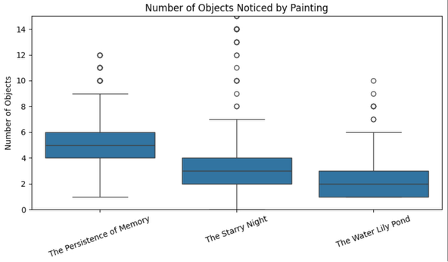
\includegraphics[width=0.4\linewidth]{Figure1.png}
    \caption{Number of objects noticed in each painting}
\end{figure}

“This art piece makes me feel sombre” is an ordinal categorical feature measured on a 5-point Likert scale (1 = Strongly disagree, 5 = Strongly agree). The stacked bar chart shows distinct response distributions across the three classes.
\begin{figure} [h]
    \centering
    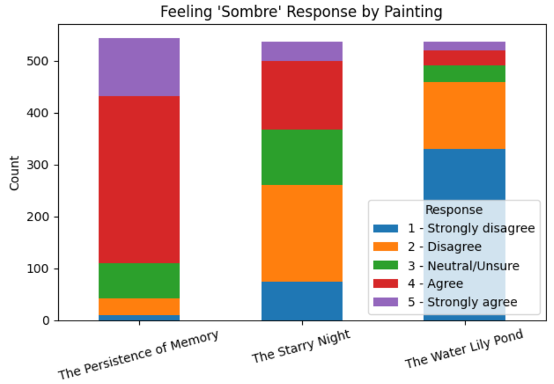
\includegraphics[width=0.3\linewidth]{Figure2.png}
    \caption{Feeling sombre response for each painting}
\end{figure}

\subsection{Model choices}
\textbf{Why Softmax Regression is Appropriate}

\begin{itemize}
    \item Key predictive features (e.g., number of objects noticed, somber score) show clear separation in central tendency across classes.
    
    \item The feature distributions suggest approximately monotonic differences rather than complex nonlinear interactions.
    
    \item Therefore, a linear decision boundary may already achieve reasonable classification performance.
\end{itemize}

\textbf{Why an MLP May Further Improve Performance}

\begin{itemize}
    \item Multi-Layer Perceptrons (MLPs) can learn nonlinear decision boundaries that logistic regression cannot capture.
    
    \item This is especially important when interactions exist across different feature modalities (textual, categorical, and numerical features), which is the case in our dataset.
    
    \item Consequently, an MLP may improve classification performance when class boundaries are not strictly linear.
\end{itemize}

\textbf{Why KNN is Appropriate as a Non-parametric Baseline}

\begin{itemize}
    \item K-Nearest Neighbors (KNN) is a non-parametric classifier that does not assume any particular shape for the decision boundary. Unlike Softmax Regression and MLP, it simply looks at the closest training examples to make a prediction.

    \item From the boxplot in Figure~1, we can see that different paintings tend to cluster in different parts of the feature space (e.g., one painting consistently gets higher ``number of objects'' responses). This means nearby points are likely from the same class, which is when KNN works well.

    \item Since we normalize continuous features and encode categorical ones during preprocessing, all features end up on similar scales, so distance-based comparisons are reasonable.

    \item KNN also serves as a sanity check, if the parametric models (Softmax, MLP) cannot beat a simple nearest-neighbour approach, that would suggest they are not learning anything useful beyond local similarity.
\end{itemize}

\newpage
% ====================================
% Methodology
% ====================================
\section{Methodology}

\subsection{Softmax Regression}

\textbf{Reason:} it is highly effective for multi-class classification with high-dimensional TF-IDF text features. The model is simple, interpretable, and robust on small datasets.

\textbf{Optimization Techniques:}
    \begin{itemize}
        \item \textbf{Optimizer}: LBFGS (or SGD)
        \item \textbf{Regularization}: L2 regularization
        \item \textbf{Learning Rate Schedule (for SGD)}: step decay or exponential decay 
        \item \textbf{Early Stopping Strategies:} Because Softmax Regression solves a convex objective using LBFGS, early stopping is not required. The optimization converges to a global minimum. For SGD, early stopping monitored the validation loss and stopped training when no improvement was observed for 5 consecutive epochs.
        
    \end{itemize}
\textbf{Validation Method:}
        \begin{itemize}
        \item \textbf{Cross-validation:} Stratified GroupKFold 5-fold cross-validation, where fold assignment respects student groups to prevent within-CV data leakage.
        \item \textbf{Hyperparameters and Rationale:}
            \begin{itemize}
                \item Optimizer: LBFGS or SGD. LBFGS works well here because the softmax objective is convex, so it converges reliably. We also try SGD since it can scale better when TF-IDF features make the input high-dimensional.
                \item L2 regularization strength $C = 1/\lambda \in \{0.1, 1, 10\}$: these three values span weak to strong regularization across orders of magnitude, covering the typical range for logistic-family models.
                \item Max iterations (LBFGS): fixed at 2000 as a safeguard, not a tuned hyperparameter, since the convex objective will converge regardless. We instead tune the convergence tolerance \texttt{tol} $\in \{10^{-3}, 10^{-4}, 10^{-5}\}$, which controls how precisely the solver needs to converge before stopping.
                \item Number of epochs (SGD only): $\{20, 30, 40\}$. Sufficient for convergence on a dataset of ${\sim}1350$ training samples.
                \item Learning rate (SGD only): $\{0.1, 0.01, 0.001\}$ with step or exponential decay. This range spans aggressive to conservative step sizes, each paired with a decay schedule to ensure convergence.
            \end{itemize}
    \item \textbf{Hyperparameter tuning process:} Grid search over the combinations above, evaluated using macro-F1 on each validation fold.
        
    \end{itemize}

\subsection{Multi-Layer Perceptrons(MLP)}

\textbf{Reason:}
Multi-layer perceptrons are suitable for this task because the dataset contains both
continuous features (emotion intensity, number of objects, number of colors) and high-dimensional categorical/text features (room preference, feelings, soundtrack descriptions, etc., after one-hot encoding or TF-IDF),
which together form a nonlinear feature space.

\textbf{Optimization Techniques:}
    \begin{itemize}
        \item \textbf{Optimizer:} Adam
        \item \textbf{Regularization:} L2 regularization
        \item \textbf{Learning Rate Schedule:}
Cosine decay or Step decay (epoch 10, 20 $\to$ learningrate $\times$ 0.1)
        \item \textbf{Early Stopping Strategies:} Early stopping monitored the validation loss and stopped training when no improvement was observed for 5 consecutive epochs.
    \end{itemize}

\textbf{Validation Method:}
        \begin{itemize}
        \item \textbf{Cross-validation:} Stratified GroupKFold 5-fold cross-validation, where fold assignment respects student groups to prevent within-CV data leakage.
        \item \textbf{Hyperparameters and Rationale:}
            \begin{itemize}
                \item Number of hidden layers $\in \{1, 2\}$: with only ${\sim}1350$ training samples, going deeper than 2 layers would likely overfit. 
                \item Hidden units per layer $\in \{32, 64, 128\}$: these sizes are standard for tabular/mixed-feature datasets of this scale; 128 is an upper bound to limit parameter count.
                \item Learning rate $\in \{0.01, 0.001\}$ with step or cosine decay: Adam's adaptive step sizes work well in this range; cosine decay smoothly anneals the rate to help convergence.
                \item L2 regularization $\lambda \in \{0.0001, 0.001, 0.01\}$: spans light to moderate weight decay to control overfitting without underfitting.
                \item Activation function $\in \{\text{ReLU}, \text{tanh}\}$: ReLU is the default choice for hidden layers due to efficient gradient flow, while tanh can sometimes work better on normalized inputs since it outputs both positive and negative values.
                \item Batch size $\in \{32, 64\}$: smaller batches introduce noise that can help regularization but slow down training; 32 and 64 are reasonable for a dataset of this size.
                \item Dropout rate $\in \{0.0, 0.1, 0.2\}$: complements L2 regularization; rates above 0.2 risk underfitting on a small dataset.
                \item Number of epochs $\in \{20, 30, 40, 60\}$: combined with early stopping (patience = 5), this gives the model enough time to converge while stopping when validation performance plateaus.
            \end{itemize}
        \item \textbf{Hyperparameter tuning process:} Grid search over the combinations above, evaluated using macro-F1 on each validation fold.
        
    \end{itemize}

\subsection{K-Nearest Neighbors (KNN)}

\textbf{Reason:} KNN classifies each test point by looking at the $k$ closest training examples and taking a majority vote. It does not assume any particular decision boundary shape, which makes it a good baseline to compare against Softmax Regression and MLP. Since it relies on distances between points rather than learned weights, it can pick up on local patterns that the other two models might miss.

\textbf{Optimization Techniques:}
    \begin{itemize}
        \item \textbf{Optimizer:} Not applicable. KNN has no trainable parameters and therefore requires no optimization procedure. 
        \item \textbf{Regularization:} The value of $k$ controls the bias--variance tradeoff: a small $k$ gives more flexible (but noisier) predictions, while a large $k$ smooths things out at the cost of potentially missing local structure. We search over a range of $k$ values to find the right balance.
    \end{itemize}
\textbf{Validation Method:}
        \begin{itemize}
        \item \textbf{Cross-validation:} Stratified GroupKFold 5-fold cross-validation (identical to the other two models), where fold assignment respects student groups.
        \item \textbf{Hyperparameters and Rationale:}
            \begin{itemize}
                \item Number of neighbours $k \in \{3, 5, 7, 11, 15, 21\}$: we use odd values to avoid ties in majority voting. The range goes from 3 (roughly 0.2\% of training samples) up to 21 (roughly 1.6\%), which covers the typical bias--variance tradeoff from highly local to more smoothed decision boundaries.
                \item Distance metric $\in$ \{Euclidean, Manhattan\}: Euclidean distance penalizes large deviations more heavily due to squaring, while Manhattan distance is more robust when some features have occasional outliers. We include both to see which works better on our mixed-feature data.
                \item Weighting scheme $\in$ \{uniform, distance\}: uniform weights all neighbours equally, while distance weighting lets closer neighbours have more influence, which can help when the class boundary falls within the neighbourhood.
            \end{itemize}
        \item \textbf{Hyperparameter tuning process:} Grid search over all combinations above, evaluated using macro-F1 on each validation fold.

    \end{itemize}

\subsection{Evaluation Metrics}
We use two complementary metrics to evaluate and compare all models:
\begin{itemize}
    \item \textbf{Accuracy} measures the overall proportion of correct predictions. Because our dataset is perfectly balanced (562 samples per class), accuracy is a meaningful primary metric that is not distorted by class imbalance.
    \item \textbf{Macro-F1 score} averages the F1 score across all three classes, where each class's F1 is the harmonic mean of its precision and recall. This is useful because accuracy alone can look fine even if the model does poorly on one particular painting, macro-F1 would drop in that case, making the problem visible. We use macro-F1 as the primary criterion when selecting hyperparameters during cross-validation.
    \item \textbf{Per-class precision and recall} are reported alongside macro-F1 to diagnose which classes, if any, are systematically misclassified.
\end{itemize}

\subsection{Model Comparison Strategy}
To make a fair comparison, we run grid search for all three models on the same GroupKFold CV splits and use macro-F1 to pick the best configuration within each family. We then compare the best version of each model side-by-side rather than tuning one model more extensively than the others. 

\newpage
        
% ===========================================
% 5. Results
% ===========================================
\section{Results}\label{sec:results}

This section should be at most 1 page.

What you should write in this section:
\begin{itemize}
  \item Report the results of your models using the evaluation metrics you described in the Methodology section, and present them clearly in tables or plots.  
  \item Analyze errors by describing common misclassifications or weaknesses, and include a confusion matrix or illustrative examples if helpful.  
  \item Compare models by summarizing performance across model families, and clearly state your final model choice as implemented in your prediction script.  
  \item Estimate test performance by \textbf{providing a single-number estimate of your best model’s accuracy on the unseen test set}. Providing a range will earn \textbf{no} marks.  
  \item Justify your performance estimate by supporting it with empirical evidence such as validation results, cross-validation stability, learning curves, or consistency across seeds/folds.  
\end{itemize}

% ================================================
% 8. Contributions and Learning
% ================================================
\section{Contributions and Learning}

This section should contain a list of 3–4 bullets, one for each student. Each student should write at most three sentences describing their main contributions and the most important lesson learned.

% ==================================================
% 9. References
% ==================================================
\section{References}

Use references whenever appropriate (e.g., when you consult textbooks, research papers, online tutorials, or external code). Cite in the text using \verb|\cite{}|. For example, let's cite the two references provided in the \texttt{.bib} file \cite{bishop2006prml,hastie2009esl}.

\bibliographystyle{plain}
\bibliography{references}

\end{document}
